
\chapter{Theoretical Background}
\label{sec:background}

This chapter provides a theoretical background with the main concepts needed for the understanding of this work. The chapter is divided into two parts: the first part provides a brief biological summary that aims to situate the reader into the research problem, its relevance, and types of data involved; the second part presents an overview of the computational aspects of the work, describing the algorithms and techniques employed. 

\section{Biological concepts}

Human cells contain a complete set of molecular instructions for life that are encoded in deoxyribonucleic acid (DNA) molecules \cite{alberts2002molecular}. DNA serves as the storage material for genetic information and is the chemical structure that transmits these instructions from one generation to the next. Each DNA molecule is composed of a sequence of nucleotides that are linked end to end, forming a long chain. These nucleotides are represented by a single-letter code that stands for the nitrogen-containing base they carry: adenine (A), guanine (G), cytosine (C), and thymine (T). 

The human genome, which is made up of a relatively small number of long DNA molecules arranged into structures called chromosomes, contains specific regions called genes that are known as the functional units of DNA \cite{simpson2022understanding}. Genes play a crucial role in encoding the instructions necessary to produce functional ribonucleic acid (RNA) molecules (noncoding RNA genes) or proteins (protein-coding genes) \cite{salzberg2018open}. The production of functional products from instructions carried by a gene is a process known as gene expression, and was formalized more than 50 years ago, when Francis Crick enunciated the central dogma of molecular biology explaining the flow of genetic information within a biological system \cite{crick1970central}.

The first step of gene expression occurs when the genetic information encoded in the DNA is used to produce an RNA molecule through a transcription process (Figure \ref{fig:protein_synthesis}). When this molecule is a messenger RNA (mRNA), it can be decoded into a protein in a second step known as translation. Although, initially, only proteins were recognized as the final functional product of gene expression, nowadays it is known that noncoding RNA molecules may also play a vital role for organisms functioning and diseases, being thus recognized as functional products of noncoding genes. Besides transcription and translation, the central dogma of molecular biology also includes a DNA replication process, in which two identical replicas of DNA are produced from a single DNA molecule.

\begin{figure*}[!th]
    \centering
      \caption{Central dogma of molecular biology \label{fig:protein_synthesis}}
    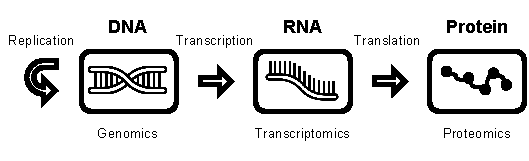
\includegraphics[width=0.87\textwidth]{images/ilustracoes/protein_synthesis.pdf}
    \legend{Source: Prepared by the author}
\end{figure*}

Proper gene function is essential for life, but when the gene sequence or activity (\ie gene expression) is disrupted by biological or environmental factors, it can lead to diseases. 
Genomic instability, which refers to an increased propensity for changes in the genome during the life cycle of cells, is influenced by genetics to varying degrees, as noted by \citet{shenzhiyuan2011}. Although all diseases are to some extent influenced by the genetic constitution of individuals, making them more or less susceptible to disorders, it is challenging to identify the genetic changes associated with a particular disease due to the vast number of variations between human genomes \cite{jackson2018}. Moreover, a disease may result from multiple variants in the DNA sequence involving one or a few nucleotides and also from environmentally induced heritable changes in gene expression that do not result from a change in the DNA sequence (known as epigenetic dysregulation).

One disease that arises from genetic and epigenetic dysregulation is cancer, a condition characterized by uncontrolled cell growth and metastasis. As there are many potential causes of cancer, the field of molecular biology is continually developing genome sequencing and computational tools to better understand cancer phenotypes and the underlying genotypic or molecular changes \cite{de2018molecular}. The next sections review relevant concepts related to the cancer genome, including the genomic changes related to the development of the disease and the types of genome-wide biological data useful for their investigation. 

\subsection{The cancer genome}

Cancer is a group of complex diseases caused by genetic changes that result in abnormal and uncontrolled cell growth \cite{stratton2009cancer}. The genetic changes may be due to inherited genetic variation or acquired somatic mutations, that is, DNA alterations that occur after conception. I classical tumorigenesis model, cancer is described as multiple and successive clonal expansions driven by the accumulation of genomic alterations that are preferentially selected by the tumor environment \cite{yates2012evolution}. These alterations may include various forms of mutations on specific genes, amplifications, deletions or rearrangements of chromosome segments, copy number changes that cause gain or loss of an entire chromosome(s), among others \cite{shenzhiyuan2011}. As a consequence, the functioning of protein-coding genes or regulatory components of the genome can be affected, particularly with regard to the control of cell growth and division \cite{stratton2009cancer}. Ultimately, cancer cells acquire the ability to invade neighboring tissues and metastasize, which makes cancer such a dangerous disease.


Since the first sequencing of the cancer genome in 2008, research has shown promising potential to advance prevention, diagnosis, prognosis, and treatment by promoting a better understanding about the fundamental biology of cancer \cite{mwenifumbo2013cancer}. An important advance was the description of several features common to most cancer cells that affect a handful of essential cellular functions and contribute to abnormal and uncontrolled cell growth, referred to as ``cancer hallmarks''. 

According to \citet{hanahan2022hallmarks}, these hallmarks comprise ``the acquired capabilities for sustaining proliferative signaling, evading growth suppressors, resisting cell death, enabling replicative immortality, inducing/accessing vasculature, activating invasion and metastasis, reprogramming cellular metabolism, and avoiding immune destruction''.

However, genome-wide analyses of tumors also revealed that cancer genome is characterized by a significant heterogeneity between and even within tumor types \cite{vogelstein2013cancer}.
The mutation load in cancer is abundant and complex - although many variations may be found between different genomes, not all of them are implicated in cancer. Moreover, it has been observed that most common cancers are associated with several genetic mutations that occur at low frequencies \cite{yates2012evolution}. Thus, one of the great challenges of cancer research is precisely discovering the ``drivers'' of the disease, such as mutations that induce tumorigenesis, and the genes whose mutated forms affect the normal functioning of a ser of essential cellular processes - known as ``cancer driver genes'' (CDGs) \cite{martinez2020compendium}. 

Cancer driver genes can be of two types based on their role in cancer progression: (i) oncogenes (OGs), which promote uncontrolled cell growth and division, or (ii) tumor supressor genes (TSGs), which prevent the cell from undergoing uncontrolled division \cite{Chandrashekar2020}. Therefore, the abnormalities in the cell cycle processes that control the tumor formation and development are due to genomic alterations that cause gain-of-function of OGs together with the loss-of-function of TSGs.


\subsection{Driver and passenger mutations}

As discussed in the previous section, the task of characterizing and understanding somatic genomic alterations and their relation with disease represents a significant challenge in cancer biology. According to \citet{stratton2009cancer}, the DNA sequence of most human cells acquire a set of differences from its progenitor fertilized egg through somatic mutations. %% types of mutations!
Somatic mutations in cancer genome may include distinct classes of DNA sequence changes \cite{stratton2009cancer}:
\begin{itemize}
    \item \textbf{Single nucleotide variant (SNV)} refers to a simple substitution of a single nucleotide for another. When this point mutation affects a coding region but does lead to amino acid substitution, the SNV is referred to as synonymous (or silent) mutation. When the nucleotide substitution alters the encoded amino acid, the SNV is called a nonsynonymous mutation. Nonsynonymous mutations can be further classified into missense or nonsense, depending on whether the nucleotide substitution results in the codon\footnote{Codon is a sequence of three consecutive nucleotides that codes for a specific amino acid.} sequence for a different amino acid that affect protein function in varying degrees (missense), or in a stop codon (nonsense) that generates truncated, incomplete, and nonfunctional protein products.

    \item \textbf{Insertion or deletions (indels)} refer to a small length of DNA (usually less than 50 base pairs) that is inserted into or deleted from the genome. When the length of the indel is not a multiple of three (\ie the length of a codon), this causes a frameshit that may drastically alter the mRNA sequence and, thus, the product of RNA translation.
    
    \item \textbf{Copy number alteration (CNA)} refers to gain or loss of large (greater than 50 base pairs) DNA sequences due to genomic rearrengements such as deletions or duplications. CNAs may encompass gene sequences, resulting in gene duplication or deletion. It is sometimes also referred to as copy number variation (CNV).
    
    
\end{itemize}

Occasionally, due to the mutations accumulated over the lifetime, a single cell may gain the capability to proliferate and survive more effectively than its neighbours. The so-called ``driver'' mutations can confer cells the advantage of growing uncontrollably, thus driving tumorigenesis.  Although it is straightforward to define a cancer driver gene as one that carries a driver mutation that provides a selective growth advantage to a cell, a plethora of somatic abnormalities present in the cell is not necessarily linked to the cancer initiation or progression. When a mutation does not provide an advantage in clonal growth and therefore does not contribute to cancer development, it is referred to as a ``passenger'' mutation \cite{vogelstein2013cancer}. In summary, a driver mutation induces uncontrolled cell proliferation and tumor growth, while a passenger mutation does not \cite{stratton2009cancer}. Since passenger mutations frequently arise during cell division, they are also present in cancer genomes, but they have no functional impact.


Therefore, the key analytical challenge in the study of cancer genome is to differentiate driver mutations from passenger mutations. Several computational strategies have emerged with the increasing availability of mutation profile data for thousands of cancer patients through initiatives such as The Cancer Genome Atlas (TCGA) or more recently, the International Cancer Genome Consortium (ICGC) \cite{hirano2020pan}. The vast amount of genomic data generated in the last years and the development of more powerful computational methods provide an excellent opportunity to predict cancer driver genes from molecular data. The next section introduces the main types of datasets explored in the prediction of cancer driver genes.



\subsection{Genome-wide biological data}
\label{sec:background:bio_data}

The identification of cancer drivers has been greatly advanced by high-throughput technologies that allow genome-wide measurements of molecular components that comprise human biological systems in any level - from DNA to proteins. This big data approach in the context of biology has generated a new field of ``omics'' science, which refers to the extensive quantification (\ie profiling) of molecular-level information spanning the whole cell or tissue of an organism \cite{li2014big}. Depending on the nature of the molecular component being measured, a different type of omics data is generated:  genomics, transcriptomics, epigenomics, proteomics, etc.  Moreover, because every component of the human system behave as part of a highly interconnected and dynamic network, multifactorial diseases like cancer are the result of disruptions in several biological and pathological processes interacting in a complex network \cite{barabasi2011network}. Thus, one way to interconnect different omics data is through biological networks, which are theoretical models that aim to represent the inherent complexity of biological systems \cite{liu2020computational}. In what follows, we review the types of omics data employed in the current work and the concept of protein-protein interaction networks. Whereas here we focus in the theoretical aspects of the biological data, in Chapter \ref{sec:materials_methods} we explain in more detail how the datasets were collected and pre-processed to be more informative for a computational prediction method.


\subsubsection{Omics data}

Since the completion of the Human Genome Project in 2003, high-throughput technologies have continued to progress and improve the rate and quality of biological data collection \cite{robinson2016integrative}. Nowadays, genome-scale measurements often replace molecule-scale measurements, allowing for investigation of the entire complement of a specific type of molecule that composes biological systems, in various levels of interrogation \cite{karczewski2018integrative}. The so-called ``omics'' data are crucial for elucidating the genomics of cancer and provide an unprecedented understanding of the molecular features underlying tumors. The Cancer Genome Atlas (TCGA) and the PanCancer Atlas have generated and analyzed omics profiling for more than 11,000 tumor samples across 33 cancer types. Among the several types of existing omics data \cite{karczewski2018integrative}, this work is interested in the following:

\begin{itemize}
    \item \textbf{Genomics}: genome sequencing assays help to determine the complete DNA sequence of organisms and to identify DNA-level changes between cancer and healthy samples. It is through genomics that different types of mutations can be characterized in their totality, such as SNVs and CNAs.
    \item \textbf{Transcriptomics}: DNA microarrays and high-throughput sequencing technologies provide the ability to measure the gene expression for the entirety of genes in an organism at the transcriptional level. Although mRNA is not the final functional product of a gene, but rather an intermediary step in gene expression, the information about transcription levels is necessary for understanding the regulatory mechanisms controling gene expression and for finding dysregulated genes associated with diseases \cite{brazma2000gene}. In transcriptomics, the complete set of RNA transcripts (\ie transcriptome) is quantified and may comprise both coding RNAs (\ie mRNA) and noncoding RNAs.
    \item \textbf{Epigenomics}: refers to the study of heritable changes in the genome that are not caused by DNA sequence mutations but still influence gene expression. The most common epigenetic mechanism is DNA methylation. DNA methylation involves the transfer of a methyl group to the C5 position of cytosine to form 5-methylcytosine \cite{moore2013dna}. DNA methylation is considered an important regulator of gene expression, causing gene silencing by recruiting proteins involved in gene repression or inhibiting the binding of the transcription factor \cite{kulis2010dna}. 
\end{itemize}


\subsubsection{Protein-protein interaction networks}
\label{sec:background_ppi}

Proteins are important building components of cells and carry out the majority of their functions. However, proteins do not function independently within a biological system; they interact with other functional components in a complex network to maintain the stability of the internal environment of cells \cite{koh2012analyzing}. Following this principle, the phenotypic impact of a disease is determined by the network context of a mutated or disregulated gene, including not only the gene itself and its function through the encoded functional products, but also its interaction partners \cite{barabasi2011network}.

There are various types of biological networks that differ in the types of macromolecules and interactions they describe. Generally, the macromolecule is represented as a ``node'' of the network and a large number of interactions, whether physical, biochemical, or functional, are represented as ``edges'' between nodes. This modeling technique provides an excellent understanding of subcellular systems on a global scale by representing the human interactome \cite{liu2020computational}. In this study, we focus solely on protein-protein interaction (PPI) networks.

PPI networks offer a valuable framework for comprehending the functional organization of the proteome, and has been frequently applied in the study of human conditions such as cancer, infectious diseases, and neurodegenerative diseases \cite{lu2020recent}. They map physical links between two or more proteins, which are represented by the nodes of the biological network \cite{liu2020computational}. To map human PPIs, there are a variety of experimental strategies, such as the yeast two-hybrid assay (Y2H), which measures direct physical interactions in cells, and affinity purification mass spectrometry, which measures the composition of protein complexes. This powerful tool can be applied in a high-throughput manner to detect these interactions in a genome-wide fashion, although at high costs \cite{stelzl2005human}. Additionally, literature-curation may be employed to systematically collect interactions from thousands of published small-scale studies targeting a single or few specific hypotheses \cite{hint}.




\section{Computational concepts}
\label{sec:comp_concepts}

Advancements in cancer genomics projects have generated massive amounts of data, providing opportunities to leverage computational approaches for more accurate prediction of cancer driver genes. A number of computational strategies have been proposed in literature, exploring several types of biological data. 
In Chapter \ref{sec:related_works}, we provide a comprehensive review of related works, summarizing these efforts under the perspective of computational methods and data employed. This section aims to present theoretical concepts that are important for building a prediction model, including the learning algorithms and the evaluation metrics adopted. 


\subsection{Machine learning and learning paradigms}


While various methods exist for prediction tasks, it is imperative to address the fundamental concept of machine learning. Machine learning (ML) is an artificial intelligence (AI) branch that allows computer algorithms to learn patterns from dat a \cite{el2015machine}. The primary goal of ML is to develop a predictive model based on statistical associations between features of a given dataset. Through this approach, ML algorithms can be explored to learn an optimal mapping between genomic features and the capacity of a given mutation or mutated gene to drive tumorigenesis. Once these predictive patterns of cancer-driving genomic variations are learned, the model can be applied in classification tasks such as discerning if a somatic mutation is a driver mutation or a passenger mutation, or if a given gene is responsible for or does not contribute to cancer. 

Considering the scope of classification tasks, ML-based models are trained to specify which of $k$ categories some input sample belongs to. The models are generated based on a given set of input data (\ie training data) that usually consists of ``features'' and ``labels'' across a set of samples. Features are the measurements across all samples, raw or mathematically transformed, while labels are the categories the model aims to predict, \ie the output of the model \cite{Camacho2018}. When the labels of the training data are known and the model aims to estimate the unknown mapping between input (\ie features) and output (\ie label) data, the ML algorithm is said to follow a supervised learning approach. The opposite of supervised learning is the unsupervised learning approach, in which only input samples are provided to the learning system and the labels are unknown.

In some situations, the labels are incomplete, that is, only a portion of the training data was previously labeled with the correct or expected outputs. Semi-supervised learning deals with problems in which the data is partially labeled. A common approach consists in using the labeled part to infer labels for the unlabeled part, and then proceed with a traditional supervised learning using the complete set of (now labeled) data \cite{el2015machine}. According to \citet{Camacho2018}, the use of semi-supervised learning may help surpass the model performance that can be achieved using only the labeled data (conducting a fully supervised learning), or ignoring the labels and considering all samples as unlabeled data in an approach known as unsupervised learning. In Chapter \ref{sec:materials_methods}, we discuss in more detail how semi-supervised learning represents an interesting perspective for predicting cancer driver genes, since many human genes still lack proper annotation for their role in tumorigenesis.

The following sections describe specific ML algorithms commonly used for classification tasks, where the model output is in the form of categories. It is worth noting that we use an organization commonly seen in the literature, grouping algorithms into traditional machine learning and Deep learning (DL) methods. 
Moreover, we highlight algorithms that are important for the experiments conducted in the upcoming chapters.



\subsection{Traditional machine learning algorithms}
\label{sec:comp_concepts:tradml}


In this section, we present some traditional ML algorithms that are commonly explored in bioinformatics and are mostly aimed at supervised learning \cite{Kotsiantis2006}. Traditional ML relies on manual feature engineering to craft features for the model. Thus, as complex as they may seem, they still demand domain expertise and human intervention. In what follows, we review support vector machine, tree-based learning algorithms, and artificial neural networks.



\subsubsection{Support Vector Machine} 

Support Vector Machine (SVM) is a powerful method for classification tasks that creates a decision boundary between two classes to predict the labels of new samples, which are comprised of one or more features. This decision boundary is a hyperplane that is oriented to be as far as possible from the closest data points of each class, which are known as the support vectors \cite{huang2018applications}.

One of the main advantages of SVM is its ability to handle non-linearly separable data using a kernel function to transform the low-dimensional space into a higher-dimensional feature space in which the problem becomes linearly separable \cite{mammone2009support}. This makes it easier to find a decision boundary that separates the classes. In essence, the kernel function is a mathematical trick that enables SVM to transform lower dimensional data into higher dimensional data with the help of new features created, and separate the points in a higher dimension. 

While there are different variations and extensions of the SVM algorithm, they all maintain the main properties that characterize the algorithm, such as the separation hyperplane, maximum margin hyperplane, and kernel function. These features allow SVM to find linear constraint problems without local maxima efficiently \cite{mammone2009support}.



\subsubsection{Tree-based learning algorithms}

Tree-based methods are a popular class of supervised learning algorithms for classification and regression tasks. These algorithms have the structure of a decision tree (DT), which divides the data recursively based on the most discriminative features and assigns a label to each region of the input feature space. Decision trees are more interpretable than other classifiers because they combine simple questions about the data in an understandable way. Other advantages of decision trees include scalability, flexibility, and less requirements regarding data preparation \cite{kotsiantis2013decision}.

Complex decision trees are prone to overfitting and, in this case, may exhibit poor generalization performance on new data. To address this challenge, pre-pruning and post-pruning techniques can be employed to control the growth of decision trees. Pre-pruning halts tree growth when there is insufficient data while post-pruning removes subtrees with inadequate data after tree construction. Nevertheless, to further address this problem, several variants of decision trees have been proposed, such as random forests and gradient boosting \cite{kingsford2008decision}.

Random forests (RF) consist of a set of decision trees, each trained on a random subset of the training data and a random subset of the features. Random samples are generated independently and with the same distribution for all trees in the forest \cite{breiman2001random}. That is, the training set is is created based on sampling with replacement through a bootstrap process to create a modified training set of the same size as the original. Furthermore, during the construction of each tree, only a small, randomly selected subset of the available resources is considered when choosing the best split at each node \cite{kingsford2008decision}. To obtain the final prediction, the algorithm aggregates the predictions of all individual trees using the majority vote \cite{breiman2001random}. The main advantages of the random forest algorithm over a single decision tree include built-in randomness that reduces overfitting and increases the diversity of individual trees. This leads to a more accurate and robust model. 



Another widely used tree-based algorithm is Gradient Boosting Trees (GBT), which combines multiple weak learners into a single stronger model. The main difference between GBT and the previous techniques is that GBT applies optimization by repeatedly re-weighting the training examples to focus on the most problematic ones. This includes a learning procedure where the objective is to construct base learners so that they are maximally correlated with the negative gradient of the loss function associated with the entire model (\ie the set of base learners) \cite{sagi2018ensemble}.

Specifically, in GBT, a sequence of regression trees is computed, where the final prediction is obtained by aggregating these predictions from all trees in an additive manner, with each added model trained to minimize the loss function. It is a powerful and versatile algorithm that can be customized and optimized for different problem domains \cite{kingsford2008decision}.


\subsubsection{Artificial Neural Networks}

Artificial Neural Networks (ANN) have become widely accepted as a powerful computational tool to solve complex real-world classification problems. ANNs are capable of modeling complex nonlinear problems, making them a popular choice in machine learning \cite{zou2009overview}. A key property of ANNs is that they are inspired by early models of sensory processing in the human brain. Thus, just as the brain is made up of an elementary unit called a neuron, artificial neurons are the fundamental building blocks of all ANN models. In essence, an artificial neuron is a mathematical function that takes in the linear combination of inputs, applies the function to them, and returns an output value \cite{krogh2008artificial}. This neural network unit is reffered to as the perceptron, which is also considered a single-layer neural network able to model only linear problems. 

The most common architecture of ANNs is the Multilayer Perceptron (MLP), which is illustrated in Figure \ref{fig:perceptron}. Neurons are arranged in sequential fully connected layers. The leftmost layer in this network is called the input layer and the neurons within the layer are called input neurons. The rightmost or output layer contains the output neurons or, as in this case, a single output neuron. The intermediary layers between the input and the output ones are known as the hidden layers. All connections among nodes in the network have their corresponding weight represented by $w$ in the figure. When designing the ANN topology, one must consider mainly , the number of hidden layers in the network and the number of nodes in each layer.


\begin{figure*}[!th]
    \centering
      \caption{Example of a Multilayer perceptron model. \label{fig:perceptron}}
    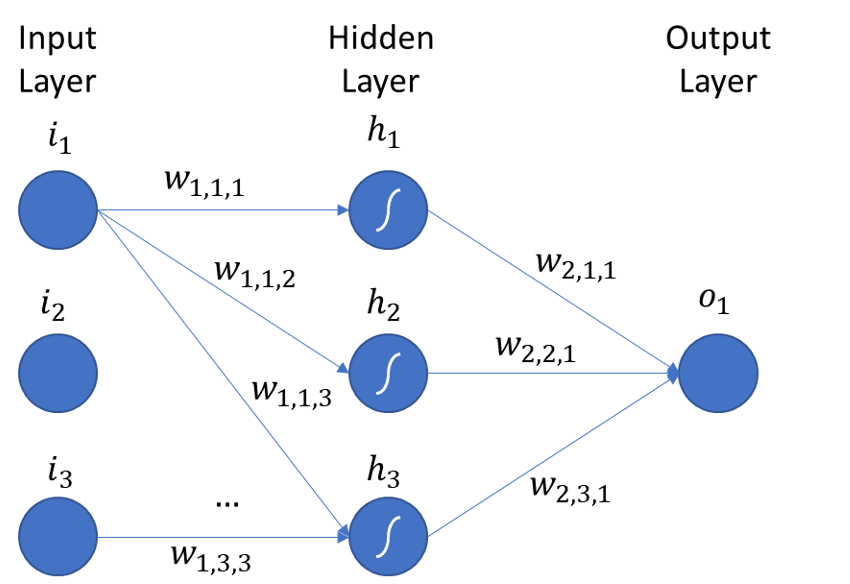
\includegraphics[width=0.65\textwidth]{images/ilustracoes/mlp.png}
    \legend{Source: \citet{trlin}}
\end{figure*}

Except for the nodes in the input layer, which propagate the original values of the input data for the subsequent layer, all other nodes implement a mathematical function that applies weights to the inputs and directs them through an activation function. These weights can be thought of as analogous to the strength of synapses in the brain. This mathematical function can be represented as follows:  

\begin{equation}
    \label{eq:neuralnetwork}
    y = \Phi \left( \sum_{i=1}^{N} (w_ix_i) + b \right)
\end{equation}
where $N$ represents the number of inputs to be processed, $x_i$ represents a single variable or input feature, $w_i$ represents a learnable weight for that input, $b$ represents a learnable bias term, and $\Phi$ represents anactivation function that takes a linear combination of the input values and returns a single output \cite{zou2009overview}. 

The activation function introduces non-linearity in the modeling process. While the sigmoid function was a traditional choice for early ANN models, other functions, such as the \textit{rectified linear unit} (ReLU), are now commonly applied due to their superior performance \cite{goodfellow2016deep}. The ReLU activation function sets negative input values to zero, while passing input values that are equal to or greater than zero. This activation function allows faster learning compared to alternatives like the sigmoid function.

During the training process, the weights of an ANN are adjusted to minimize the total error between its output and the desired output (\ie the labeled data). These weights are typically initialized with small random values, and the training involves measuring the square difference between the ANN output and the desired output for each input, with the goal of minimizing the sum of these differences as much as possible. Backpropagation, a gradient-based optimization algorithm, is commonly used to adjust the weights by propagating the errors back through the network \cite{krogh2008artificial}.



\subsection{Deep learning and graph-based learning}
\label{sec:deep_and_gnns}

The field of bioinformatics is experiencing an increase in the accumulation of omics data through experimental studies. While traditional ML algorithms, such as ANNs, have been widely used to extract knowledge from this data, the emergence of big data has led to the development of more advanced and complex model architectures. Although these architectures are still based on ANNs, there has been a shift in focus towards deep learning (DL), which has shown promising results in achieving higher accuracy and performance compared to traditional ML algorithms. Consequently, DL has generated significant interest in academic and research communities. According to \citet{min2017deep}, this growth can be attributed to the advances made in deep learning, which have contributed to the growth of both sub-areas, as illustrated in Figure \ref{fig:min2017deep}.

\begin{figure*}[!th]
    \centering
      \caption{Number of published deep learning articles by year. \label{fig:min2017deep}}
    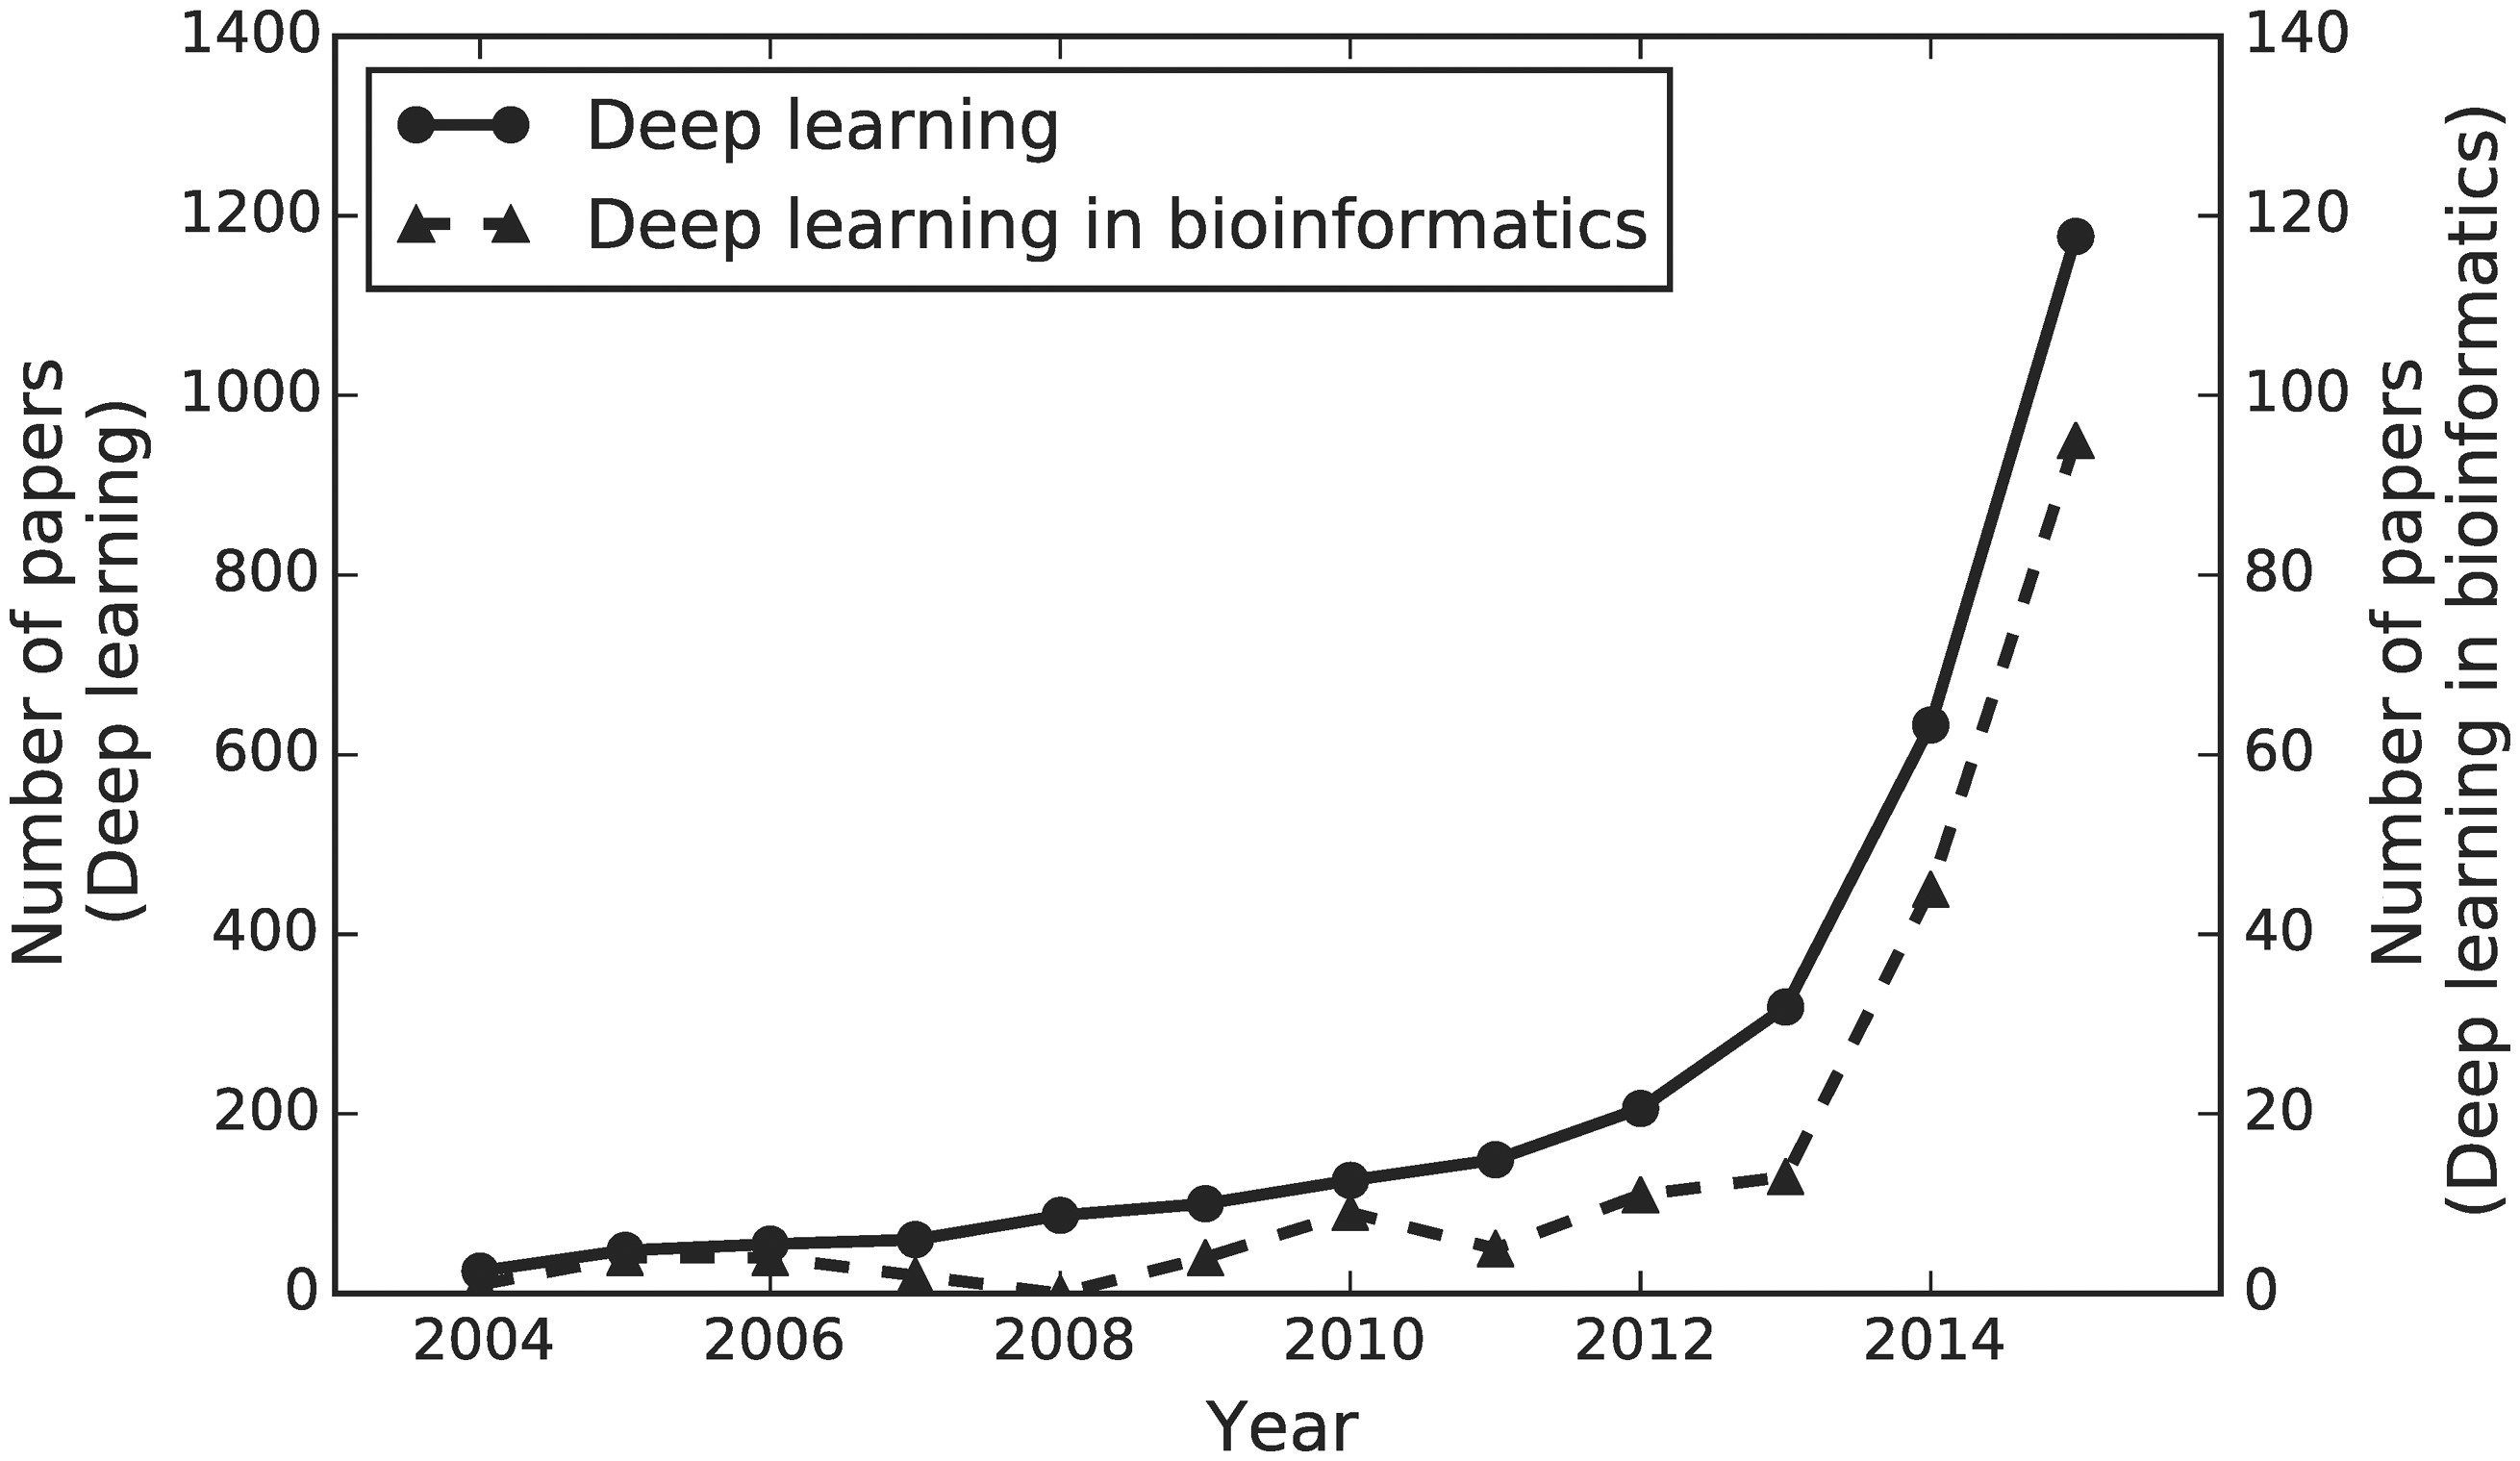
\includegraphics[width=0.9\textwidth]{images/ilustracoes/min2017deep.jpeg}
    \legend{Source: \citet{min2017deep}}
\end{figure*}

The success of deep learning can be attributed to the significant algorithmic detail involved in both constructing and training its architectures. Typically composed of multilayer artificial neural networks that leverage non-linear transformations, these architectures take on various forms depending on the characteristics of the input data and research objectives. Deep learning, as a subfield of ML, employs hierarchical architectures to learn high-level abstractions in data, enabling more accurate and sophisticated predictions and insights to be made from the data \cite{goodfellow2016deep}.



One of the most representative network architectures in the field of deep learning is the convolutional neural network (CNN), which is designed to process data in matrix format. CNNs can be seen as a sequence of convolution layers and pooling layers. The convolution operation is implemented through the application of filters in the input. The filters are defined as a matrix of weights with the same values repeated in a specific order that is multiplied by the input. During this operation, specific characteristics are retained from the input while others are ignored, depending on the filter applied. The result of the convolution is usually passed through a non-linear activation function such as ReLU \cite{li2021survey, lecun2015deep}. The convolution layer can be followed by a pooling layer that applies the poolin operation. In this step, groups of adjacent values in the input data (for example, groups of 2x2 pixels in an image) are aggregated by taking the maximum value among the (\ie Max Pooling) or the average among them (\ie Average Pooling). Pooling operations have the utility of intensifying important characteristics or features identified in the convolution layer. 

Despite the effectiveness of CNNs in modeling regularly structured information, several domains produce data with irregular structure in non-Euclidean space. Graphs, which provide an effective representation of entities and their relationships, are among the many irregular geometric shapes commonly encountered in these domains \cite{georgousis2021graph}. Graphs are well-suited to modeling complex structures such as protein-protein interactions, which are natural networks found in the biological domain, as discussed in Section \ref{sec:background_ppi}. In what follows we provide basic definitions of graph structures and we introduce adaptations in deep learning algorithms to allow learning from graphs.




\subsubsection{Basics of graph theory and node centralities}
\label{cap:basis_graph_centralities}


A graph is a mathematical structure comprising a set of vertices (or nodes) and edges that connect them. We represent a graph as a pair of vertices (V) and edges (E), denoted as $G = (V, E)$. An edge that links two vertices $i$ and $j$ may optionally have a weight $w_{ij} \in \mathbb{R}$ assigned to it. Depending on whether each edge has a weight assigned to it or not, a graph can be either weighted or unweighted. Likewise, a graph can be either directed or undirected, depending on whether its edges have a specific direction. For instance, protein-protein interactions can be represented as graphs, where nodes depict proteins and edges depict physical or functional connections among them. When a graph is weighted, the weights can signify the confidence level of the existence of a given connection between proteins.



Among the many utilities in using graph-based representation, the analysis of centrality measures are among the most widely used applications. Centralities are crucial features of graphs and help to identify the most influential or central nodes. Four centrality measures are of special interest in this work:

\begin{itemize}
  
    \item \textbf{Degree}: is the number of neighbors of a node $i$ in the network, or in other words, the number of edges that are incident on a given node, considering an undirected graph.

    \item \textbf{Betweenness}: quantifies the number of times that a given node is needed for any node to reach any other node in the graph. Nodes that appear more frequently along the shortest paths between other nodes will receive higher betweenness centrality scores. It is a way of detecting the influence that a node has on the flow of information in a graph based on the extent to which it lies on the shortest paths between pairs of other nodes.

    \item \textbf{Closeness}: computes the sum of distances from a given node to all other nodes, based on the shortest paths between all pairs of nodes. The resulting sum is then inverted to determine the closeness centrality score for that node. In the case of disconnected graphs, where there may not be a path between every pair of nodes, the number of nodes is used as a substitute for the length of the geodesic, which always results in a longer path than the longest possible geodesic. 

    \item \textbf{Clustering coefficient}: also called transitivity, is defined as the ratio of the number of edges between the node's neighbors over the maximum possible number of such edges. The transitivity of a graph is then defined as the average of the clustering coefficients of all its nodes. In case of the local transitivity, this probability is calculated separately for each node. 
\end{itemize}




These different types of centralities can be used in various contexts to understand the structure and behavior of networks and to identify important nodes for distinct applications.





\subsubsection{Introduction to graph neural networks}
\label{sec:backgroud:gnns}

To extend the application of convolution and pooling operations from regular grids to arbitrary graphs, it is necessary to recognize that the connectivity patterns in graphs, specially those deriving from biological networks, are typically irregular. Graphs do not exhibit the regular structure found in images, thus presenting a challenge for deep learning algorithms \cite{chen2020simple}.


Graph Neural Networks (GNNs) are a promising approach to address the complexity of such patterns by extending the structural principles of CNNs to non-Euclidean data. In GNNs, a filter is applied to each node in the graph and its neighboring nodes, allowing the recognition of patterns in the local neighborhood of a node and the extraction of local structural information from the graph. This enables GNNs to learn representations of graph-structured data and perform various tasks such as node classification, link prediction, and graph-level prediction \cite{zhang2019graph}.

In the process of selecting a GNN model, some crucial steps must be considered. One such step is determining the type of graph structure, which can be divided into two scenarios: structural and non-structural. In structural scenarios, the graph's structure is explicit in the applications, whereas in non-structural scenarios, the graph is implicit, and it must be built from the task at hand. After obtaining the graph structure, the type of graph must also be determined. As previously mentioned, graphs are typically categorized as either directed or undirected, with directed graphs having edges that are directed from one node to another. Additionally, graphs can be classified as either homogeneous or heterogeneous, with homogeneous (heterogeneous) graphs having nodes and edges of the same (different) types. Moreover, it is also important to define the loss function based on the type of learning task addressed (\ie at node-level, edge-level, or graph-level prediction).



A GNN model is usually built based on the combination of computational modules, which commonly include the propagation module, the sampling module, and the pooling module \cite{zhou2020graph, georgousis2021graph}. The propagation module is particularly important for our work, as it enables the dissemination of information between nodes, allowing for the aggregation of both features and topological information to create embeddings. The sampling module is typically used in conjunction with the propagation module when the graphs are large and need to be separated into modules. Finally, the pooling module is employed to extract information from nodes when representations of subgraphs or high-level graphs are required.


The propagation modules in GNNs typically consist of three subcomponents: the convolution operator, the recurrent operator, and the jump connection, as discussed by \citet{zhou2020graph}. In this text, we will focus on the most commonly used subcomponent for GNN models, the convolution operator, which aims to generalize convolutions from other domains to the graph domain.

Graph convolutions have shown successful applications in various fields, including bioinformatics, where they are particularly useful for analyzing data with no clear and visible structure, such as protein-protein interactions \cite{eraslan2019deep}. Existing graph convolution models can be broadly classified into two categories: spectral-based and spatial-based. Spectral-based models utilize principles from graph signal processing, such as the Laplacian and Fourier transform, to map the irregular structure of a graph onto a regular Euclidean space, enabling convolutional operations. In contrast, spatial-based models directly define the convolution operation using the information dissemination mechanism inherent in the graph, with propagation methods similar to those of standard CNNs. 

\begin{figure*}[!th]
    \centering
    \caption{Algorithms selected under computational module}
    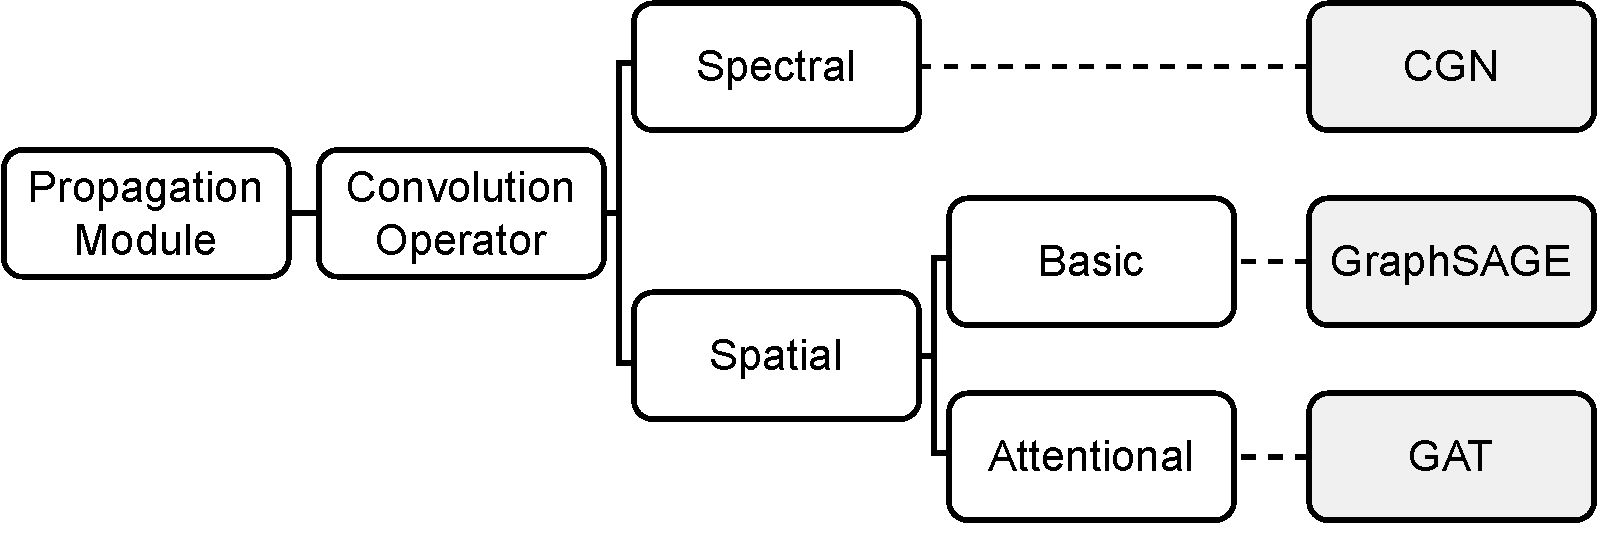
\includegraphics[width=0.80\textwidth]{images/ilustracoes/gnn_modules2.pdf}
    \legend{Source: Adapted from \citet{zhou2020graph}}
    \label{fig:gnn_modules}
\end{figure*}

The GNN algorithms selected for exploration in this work are presented in Figure~\ref{fig:gnn_modules}, adapted from \citet{zhou2020graph}. These algorithms are part of the propagation modules, which are responsible for propagating information between nodes, allowing for the capture of topological and feature-related data. This aligns with the goals of our work, which aims to leverage the structure of PPI networks and the information contained in omics data for identification of CDGs, which can be modeled as a node prediction task. As such, these algorithms are ideal constructs for the design of our predictive model. The next sections briefly explain these algorithms



\subsubsection{Spectral-based models: Graph Convolutional Networks}

Spectral graph theory provides the foundation for graph convolution in the spectral domain, which involves transforming graph signals from the nodes domain to the spectral domain. By applying a Fourier or wavelet transform to the signal using the graph Laplacian, spectral approaches can convert graph signals to the graph's frequency domain or spectrum, allowing local convolutions using shared weights similar to traditional CNNs \cite{georgousis2021graph}.

Graph Convolutional Networks (GCN), proposed by \citet{kipf2016semi}, are based on the idea that the properties of a node within a network are substantially influenced by its neighboring nodes' attributes (\ie features). The model aims to learn a function of signals/features in a graph $G = (V, E)$ that takes as input a feature matrix $X = N \times D$ and an adjacency matrix $A$ representing the graph structure. The output is a node-level matrix $Z$ of size $N \times F$, where $F$ is the number of output features per node. Each neural network layer can be expressed as a non-linear function:


\begin{equation}
\label{eq:non_linearfunc}
{H}^{(l+1)}=f(H^{(l)},A)
\end{equation}
where $H^{(0)} = X$ and $H^{(L)} = Z$ (where $L$ represents the number of layers). The different models vary only in how the function $f$ is selected and parameterized.


The layer propagation rule can be represented by:

\begin{equation}
\label{eq:pro_rule}
f(H^{(l)}, A) = \sigma(AH^{(l)}W^{(l)})
\end{equation}
where $W$ is a weight matrix for the $l$-th neural network layer, and $\sigma$ is a non-linear activation function like ReLU.


Enforcing self-loops in the graph is a common approach to guarantee that each node propagates its own feature vector. This is done by simply adding the identity matrix to $A$. However this $A$ is typically not normalized and therefore multiplying with will completely change the scale of the feature vectors. To solve this problem, it is necessary to guarantee the normalization of $A$ so that all lines add up to one, that is, $D^{-1}A$, where $D$ is the diagonal node degree matrix. Multiplying with $D^{-1}A$ corresponds to taking the average of neighboring node features. And when we use a symmetric normalization $D^{-\frac{1}{2}}AD^{-\frac{1}{2}}$ we essentially arrive at the propagation rule introduced by \citet{kipf2016semi}: 

\begin{equation}
    \label{eq:pro_rule_final}
    f(H^{(l)},A) = \sigma(\hat{D}^{-\frac{1}{2}}\hat{A}\hat{D}^{-\frac{1}{2}}H^{(l)}W^{(l)})
\end{equation}
with $\hat{A} = A + I$, where $I$ is the identity matrix and $\hat{D}$ is the diagonal node degree matrix of $\hat{A}$.


Figure \ref{fig:gnn_ilustracao} illustrates the input channels (C) and the feature maps (F) in the output layer of a spectral-based graph convolution \cite{zhang2021graph}.

\begin{figure*}[!th]
    \centering
      \caption{Schematic depiction of a graph convolution model. \label{fig:gnn_ilustracao}}
    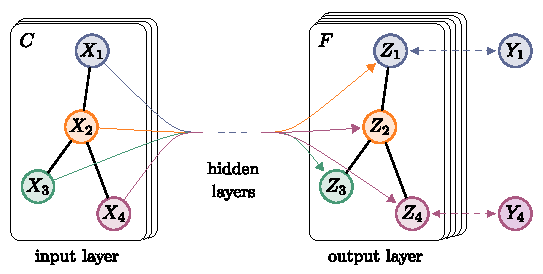
\includegraphics[width=0.8\textwidth]{images/ilustracoes/gnn_ilustracao.pdf}
    \legend{Source: \citet{kipf2016semi}}
\end{figure*}



    
\subsubsection{Spatial-based models: Graph Attention Networks and GraphSage}

Spatial convolution on a graph is similar in concept to convolution on a regular domain. Spatial techniques define convolutions directly on the graph, leveraging its topology. However, the challenge lies in devising a convolution operation that can accommodate varying neighborhood sizes while preserving the local invariance of Convolutional Neural Networks (CNNs) \cite{zhou2020graph}.


To address the limitations of Graph Convolutional Network (GCN) and other structurally similar models, Graph Attention Network (GAT) was proposed by \citet{velivckovic2017graph}. GAT incorporates an attention mechanism during the graph propagation stage to learn the edge weights between connected nodes. The GAT model takes the node feature set $x = \left\{ x_1, x_2, ..., x_n \right\}$ as input to an attention layer, which outputs a new set of learned node features $h = \left\{h_1, h_2, ..., h_n\right\}$. The attention coefficient for the edge $(i,j)$ is denoted by $\alpha_{ij}$ and is defined by the following equation:
\begin{equation}
    \label{eq:gat_equ1}
    \alpha_{ij} = \frac{exp(LeakyReLU(a^T[Wx_i||Wx_j]))}{\sum_{k\in N_i}exp(LeakyReLU(a^T[Wx_i||Wx_k]))}
\end{equation}
here, $N_i$ refers to the set adjacent nodes of node $i$, $a$ denotes the learnable weight vector, and $W$ is the shared linear transformation weight matrix. The output features for each node are computed using the following equation:

\begin{equation}
    \label{eq:gat_equ2}
    h_i = \sigma(\sum_{j\in N_i}\alpha_{ij}Wx_j)
\end{equation}

The technique of multi-head attention extends the attention layer to $K$ separate attention mechanisms, thereby promoting the stability of the self-attention learning process. Figure \ref{fig:gat_ilus_B} illustrates how the algorithm operates. The final expression is provided as follows:

\begin{equation}
    \label{eq:gat_equ_final}
    h_i = \sigma(\frac{1}{K}\sum_{k=1}^{K}\sum_{j\in N_i}\alpha_{ij}^{k}W^kx_j)
\end{equation}

\begin{figure*}[!th]
    \centering
      \caption{Multi-head attention (with $K = 3$ heads) by node 1 on its neighborhood.}
    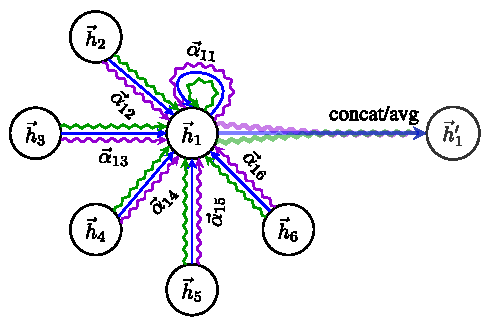
\includegraphics[width=0.70\textwidth]{images/ilustracoes/gat_ilus_B.pdf}
    \legend{Source: \citet{velivckovic2017graph}}
    \label{fig:gat_ilus_B}
\end{figure*}


    % GraphSAGE

\citet{hamilton2017inductive} proposed another spatial-based model that uses a conceptually simpler GCN, referred to as GraphSAGE (SAmple and aggreGatE). This model is a general inductive framework that leverages node attribute information to generate node embeddings for previously unseen data efficiently. Instead of training separate embeddings for each node, a function is learned that generates embeddings by performing sampling and aggregation of features from a node's immediate neighborhood.

Each layer of the GraphSAGE network consists of two principal procedures: sampling and aggregation. The aggregation procedure for a layer $l$ also consists of two steps. The first step is the aggregation of the signals from a node's immediate neighborhood:
\begin{equation}
    \label{eq:sage_equ1}
    \mathrm{h}_{N_i}^{l+1} = aggregate_{l+1}(\left\{ {h}_{j}^{l}, \forall j \in N_i \right\})
\end{equation}

The second step is the concatenation of the aggregated signals with the target node signal, which is passed through a dense layer: 

\begin{equation}
    \label{eq:sage_equ2}
    \mathrm{h}_{i}^{l+1} = \sigma(W^{l+1} .[{h}_{j}^{l} || {h}_{N_i}^{l+1}])
\end{equation}
where $W_l \in \mathbb{R}^{d\times 2c}$ is a matrix of learned weights for the $l$th layer, and $\sigma$ is a non-linear activation function, and the first layer $h_0$ is the imput signal.


\subsection{Ensemble learning}
\label{sec:comp_concepts:ensemble}

Ensemble learning is a popular approach in machine learning that involves combining multiple individual models to improve overall predictive performance, particularly in supervised tasks. Once the individual models, also known as base learners or base models, are trained, their combined predictions can be used to label new, unseen data. The central idea behind ensemble learning is that introducing diversity among models, whether through variations in data or algorithms, can compensate for errors in individual models and improve overall performance more effectively than a single model \cite{sagi2018ensemble, dong2020survey}.

Building an ensemble model involves, in general, applying a methodology for training the individual models in order to introduce some degree of diversity among them, and choosing a suitable process for combining the outputs of these models into a single output. Diversity can be introduced, for example, by random resampling the data or by employing different learning algorithms or different hyperparameters configuration. Regarding the combination of the results from the base models, although several approaches exist, they can be organized into two main categories:

\begin{itemize}

    \item \textbf{Strategies that combine the predicted class labels}: each base model provides a class label that is meaningful to the problem domain. A simple, yet very effective approach to combine these predictions, is by voting. The majority voting method, for instance, involves predicting the class label with the most votes. 
    
    \item \textbf{Strategies that combine the predicted class probabilities}: most ML algorithms are able to assign a probability for each class, which summarizes the likelihood of an instance belonging to that class. Thus, combination rules for ensemble models can also be applied over the predicted probabilities. One common way to merge probabilities is simply to take the average among values predicted for a given class. Then, the ensemble class label can be extracted based on the class that maximizes the merged probabilities.
    
\end{itemize}
We note that the algorithms Random Forest and Gradient Boosting Trees, presented in Section~\ref{sec:comp_concepts:tradml}, are examples of ensemble-based learning methods. RF introduces diversity by applying a repeated resampling without replacement (\ie bootstrap), while GBT uses a boosting strategy that resamples data based on weights that are adjusted throughout the process according to previous classification hits and errors.




\subsection{Class imbalance}
\label{sec:background_ClassImbalance}

Class imbalance occurs when there is an uneven distribution of instances across the target classes in a classification problem. The majority class has the highest proportion of instances, while the minority class has the fewest, resulting in limited representation for the concept underlying the minority class in the dataset \cite{he2009learning}. In many cases, the minority class is of particular interest, such as in clinical diagnosis with ML predictive models, where only a small fraction of patients are expected to present the disease, or when predicting cancer driver mutations, where most sequenced mutations are passenger rather than driver mutations.

Although several real world problems are characterized by class imbalance in their data distribution, when the training data is imbalanced, ML algorithms struggle to distinguish effectively between the minority and majority class. This happens because most standard ML algorithms expect balanced class distributions or assume equal misclassification costs (\ie the cost of a false positive prediction is the same as of a false negative one) \cite{he2009learning}. Thus, class imbalance presents a longstanding challenge for ML, as models tend to be biased towards the majority class, leading to high error rates for the minority class \cite{leevy2018survey}. 

Several class imbalance learning solutions have been proposed in literature \cite{he2009learning}. In what follows, we briefly review those employed in the current work:
\begin{itemize}
    \item \textbf{Undersampling Majority Class}: a widely used approach that involves a direct subsampling technique to balance class distributions. The technique randomly excludes instances of the majority class, usually until this class has the same number of instances as the minority class. This technique is only suitable for large datasets as it can potentially discard crucial data points for the model.

    \item \textbf{Balanced Cross-Entropy}: a popular technique to tackle class imbalance that involves introducing a weighting factor, denoted as $\alpha \in [0, 1]$ for the positive class and $1 - \alpha$ for the negative class. This weight factor represents an attempt to readjust the misclassification costs. In practice, $\alpha$ can be determined by the inverse class frequency or treated as a hyperparameter and determined through cross-validation. The $\alpha$-balanced cross-entropy (CE) loss can be expressed as follows:

    \begin{equation}
    \label{eq:cross_entropy}
    CE(p_t) = -\alpha_t log(p_t)
    \end{equation}
    where $p_t$ is the model’s estimated probability $p$ for the positive class if the observed class is actually positive

    \item \textbf{Focal Loss}: a newer approach proposed by \citet{lin2017focal}, which is a dynamically scaled cross-entropy loss encompassing a scaling factor that gradually decreases to zero as the confidence of the model in the correct class prediction increases. This scaling factor $(1 - p_t)^\gamma$ can effectively reduce the influence of simpler examples during the training phase and facilitate the model to concentrate on more complex examples. Thus, the $\alpha$-weighted FL for binary classification is defined as shown by the equation below:

    \begin{equation}
    \label{eq:focal_loss}
    FL(p_t) = -\alpha_t(1-p_t)^\gamma log(p_t)
    \end{equation}
    where $\alpha$ is the same weighting parameter used in balanced cross-entropy, while $\gamma$ is a new adjustable parameter that controls the degree of focusing. When $\gamma = 0$, the function is equivalent to the balanced cross-entropy approach.
\end{itemize}





\subsection{Model evaluation}
\label{sec:background_modelEvaluation}


Model evaluation is a critical step in a machine learning pipeline and is typically applied to three main sub-tasks in model development \cite{raschka2018model}: (i) estimate the generalization performance of a trained model, that is, assess the predictive performance of the model on future (unseen) data, (ii) increase the predictive performance of a learning algorithm by exploring the hypothesis space more broadly with different hyperparameter settings (\ie conduct a fine-tuning of hyperparameters), and (iii) select the ML algorithm that is best-suited for our prediction problem (\ie compare different algorithms). The step of model evaluation entails two main decisions: how to split the original dataset to allow model training and performance assessment, and how to evaluate the predictive performance. The next sections review concepts related to these aspects.

\subsubsection{Data splitting strategies}

The holdout method is a simple and commonly used data splitting strategy in machine learning. It involves randomly dividing a labeled dataset into two parts: a training set and a test set, typically in a 75:25 ratio (other common ratios are 70:30 and 80:20). The training set is used to fit the model, while the test set is used to evaluate its performance on unseen data. To ensure that the resulting subsets are representative of the original dataset, random splitting is often conducted in a stratified manner, preserving the original class proportions in the resulting subsets. Although widely adopted for model evaluation, holdout method presents some limitations: (i) it is very sensitive to how we split the data into training and test sets, (ii) it does not allow us to estimate how performance varies according to differences in the test set, (iii) it does not support the hyperparameter optimization process, which must be done with independent data to avoid the effect of data leakage \cite{raschka2018model}.


To address these limitations and provide a more robust estimate of performance, $k$-fold cross-validation (CV) has become the most common technique for model evaluation and selection in ML. The idea of $k$-fold CV is to split the dataset into $k$ disjoint parts (\ie folds) of similar size: one part is used for validation, and the remaining $k - 1$ parts are merged into a training set in an iterative process. Although $k$ is a hyperparameter of the algorithm, $k = 5$ and $k = 10$ are commonly applied values. At the end, the performance is usually estimated as the arithmetic mean (and standard deviation) over $k$ validation sets. Through this process, $k$-fold CV guarantes that all instances are used for training and testing, reducing the risks of a highly pessimistic or optimistic performance estimate.

Holdout and $k$-fold CV are often used together for model evaluation and selection. In this approach, holdout is applied as a first step to split the original dataset into training and test sets. The test set is kept aside as an independent dataset from the process of model training and selection to avoid data leakage. The training set is then used in the $k$-fold CV to experiment with one or more algorithms and various hyperparameter settings. The resulting performance estimates from $k$-fold CV are used to select the best hyperparameter setting for the algorithm, which is then used to fit the model with the complete training data. Finally, the independent test set withheld in the first step is used for the final evaluation of model performance.


\subsubsection{Performance metrics for classification tasks}


Several performance metrics can be adopted to assess distinct types of correct predictions (\ie true positive (TP) and true negative (TN)) and incorrect predictions (\ie false positive (FP) and false negative (FN)) in binary classification tasks. Here, we summarize the metrics analyzed in the current work.

\begin{itemize}
    \item \textbf{Accuracy} (\textbf{Acc}): reflects the proportion of instances in the test set that were predicted correctly by the model (\ie the hit rate). Accuracy alone may not properly reflect the model performance for datasets with class imbalance, especially in severily skewed data distribution, as it may be biased towards the majority class. The metric is computed as follows:
    \begin{ceqn}
    \begin{align}
        Acc = \frac{TP + TN}{TP + FP + TN + FN}
    \end{align}
    \label{eq:accuracy}
    \end{ceqn}
    
    \item \textbf{Precision} (\textbf{Prec}): estimates the proportion of positive instances predicted correctly by the model. Precision is also called Positive Predictive Value (PPV) and is a measure of classifiers exactness.  Low precision indicates a high number of false positives. Precision is computed according to the following equation: %
    \begin{ceqn}
    \begin{align}
        Pre = \frac{TP}{TP + FP}
    \end{align}
    \label{eq:precision}
    \end{ceqn}
    
    \item \textbf{Recall} (\textbf{Rec}):  measures the ability of a model to correctly identify positive instances. Recall is also called Sensitivity or True Positive Rate (TPR), and a low recall indicates a high number of false negatives. Recall is estimated as follows:
    \begin{ceqn}
    \begin{align}
        Rec = \frac{TP}{TP + FN}
    \end{align}
    \label{eq:recall}
    \end{ceqn}
 
    \item \textbf{Specificity} (\textbf{Spe}): measures the proportion of true negatives that are correctly identified by the model. Specificity is also called True Negative Rate (TNR), and is computed according to the following equation:
    \begin{ceqn}
    \begin{align}
        Spe =\frac{TN}{TN + FP}
    \end{align}
    \label{eq:especificidade}
    \end{ceqn}
    The sum of specificity and false positive rate (FPR) is always 1. Thus, it is common estimate the FPR as:
        \begin{ceqn}
    \begin{align}
        FPR = 1 - Spe
    \end{align}
    \label{eq:fpr}
    \end{ceqn}
\item \textbf{Area under the ROC curve} (\textbf{AUC-ROC}): the Receiver Operator Characteristic (ROC) curve shows the trade-off between true positive rates (\ie sensitivity, in the y-axis) and false positive rates (in the x-axis) across different thresholds of prediction probability\footnote{Most performance metrics evaluate classifiers based on a specific probability threshold, usually 0.5, meaning that an instance is assigned to the positive class if the predicted probability is equal or above 0.5. This is the case, for instance, for accuracy, precision, recall, and specificity. When using approaches based on performance curves, the skill of a model is assessed across all thresholds of probability.}. The area under the generated ROC curve (AUC-ROC) is often used as an estimate of model performance and represents the probability that a randomly chosen positive instance will be ranked higher than a randomly chosen negative instance. Thus, the higher the AUC-ROC value, the better the predictive performance of the model. 
\item \textbf{Area under the Precision-Recall curve} (\textbf{AUC-PR}): the Precision-Recall (PR) curve shows the tradeoff between precision (\ie in the y-axis) and recall (in the x-axis) for distinct thresholds of prediction probabilities. The area under the PR curve (AUC-PR) is very useful to summarize the performance, with high scores meaning that the model is able to return precise results (high precision), as well as to correctly predict the majority of the positive instances (high recall).  
The AUC-PR is a more appropriate measure of classification success under the presence of class imbalance.

\end{itemize}
